\long\def\/*#1*/{}
\chapter{Pierwszy problem NP}

\section{Wstęp}

Aby przejść do rozważań nad konkretnymi problemami z klasy NP-zupełnej należy wpierw skupić się nad znaczeniem tej klasy. W teori NP-zupełności fundamentalne znaczenie ma metoda redukcji pomiędzy dwoma problemami. Podstawą wykorzystania tej metody jest założenie że klasa ta jest niepusta dzięki czemu możemy pokazać redukcję problemu, który chcemy wprowadzić do tej klasy względem problemu znajdującego się już w klasie NP-zupełnej. Jak widać początki zawsze są najtrudniejsze z tej racji “jak tego dokonać jeśli w początkowych rozważaniach klasa NPC jest pusta?”. Oczywiście nie można posłużyć się redukowalnością, aby wprowadzić pierwszy “pierwotny” problem. Niezbędne okaże się skorzystanie wprost z definicji, by w ten oto sposób zasilić klasę NP-zupełną o pierwszy problem. Później w oparciu o to będziemy mogli już redukcją wprowadzać pozostałe problemy.

\section{Charakterystyka klasy NP-zupełnej}

Definicja NP-zupełności mówi że, aby problem należał do klasy NPC musi spełniać dwa warunki, które można sprowadzić do następujących własności:
\begin{enumerate}
\item świadectwo problemu jest weryfikowalne w czasie wielomianowym
\item jest co najmniej tak "trudny", jak każdy problem z NP.
\end{enumerate}

Własność 1. nie wydaje się względnie trudnym warunkiem, natomiast warunek 2., choć wygląda niepozornie może przysporzyć wielu kłopotów. Własność ta mówi o tym, że każdy problem z klasy NP można zredukować do naszego problemu. Tu zaczynają się komplikacje, ponieważ jesteśmy zmuszeni do określenia metody redukcji każdego problemu z klasy NP (nie ważne jaki on by nie był) do naszego problemu “pierwotnego”. Choć pozornie to zadanie wydaje się nie do zrealizowania o tyle istnieje na to bardzo ciekawe rozwiązanie. Błyskotliwe spostrzeżenie będące rozwiązaniem naszej zagadki jest ukryte w komputerach, a dokładnie na relacji pomiędzy modelem danych, a jego niższą warstwą fizycznych danych. Oczywiste jest to, że algorytmy implementujemy w pamięci komputera, zaś ten jest w stanie przeprowadzić jego działanie, tak aby otrzymać wynik. Natomiast cała idea tego przetwarzania jest realizowania na gigantycznych sieciach logicznych. Przyjrzyjmy się zatem problemowi spełnialności układów logicznych jako potencjalnemu kandydatowi na rolę “pierwotnego” problemu w klasie NPC.

\section{Problem spełnialności układów logicznych}

Problem spełnialności układów logicznych (CIRCUIT-SAT) to układ $C$ zbudowany ze stałej liczby wejść binarnych oraz bramek logicznych. W podstawowym charakterze wyróżniamy bramki AND, OR I NOT. Układ nazywamy spełnialnym jeśli istnieje takie wartościowanie wejść sprawiające iż po wykonaniu wszystkich operacji logicznych z bramek na wyjściu otrzymamy prawdę.

Chcąc znaleźć rozwiązanie tego problemu istniej jedynie najbardziej prymitywny sposób jego realizacji. Polega on na sprawdzeniu wszystkich możliwych odpowiedzi, a dokładniej w obecnym tu przypadku na zbadaniu wszystkich możliwych wartościowań wejścia układu. Zakładając że układ składa się z $k$ wejść od razu widać że należy sprawdzić $2^{k}$ możliwych przypadków niezależnie od rozmiaru egzemplarza danych wejściowych. Sprawia to, że czas działania takiego algorytmu jest wykładniczy, czyli wyższy od wielomianowego.

Spróbujmy wykazać teraz, że CIRCUIT-SAT $\in$ NPC. W tym celu wpierw skupmy się na pierwszej własności i udowodnijmy, że pozytywne świadectwo można weryfikować w czasie wielomianowym, czyli w rezultacie CIRCUIT-SAT $\in$ NP.

\begin{lem} 
CIRCUIT-SAT $\in$ NP
\end{lem}

\begin{proof}
Algorytm weryfikujący problem CIRCUIT-SAT na wejściu oczekuje dwóch parametrów. Pierwszy to egzemptlarz $E$ pełnej specyfikacji układu logicznego $C$, natomiast drugi parametr to świadectwo $y$ zawierające binarne wartości przypisane do konkretnych wejść. Pierwszym krokiem algorytmu jest sprowadzenie układu logicznego $C$ do zapisu w formie odwrotnej notacji polskiej. W tym procesie bramki logiczne zostają przekształcone na operandy logiczne w następujący sposób: AND jako koniunkcja, OR jako alternatywa, a NOT negacja. Przy rozsądnej specyfikacji układu logicznego krok ten można wykonać w sposób liniowy. Następną czynnością jest wykonanie tych operacji względem wartości logicznych z świadectwa $y$. Do uzyskania poprawnej kolejności wykonywanych operacji na bitach wykorzystuje się strukturę kolejki i stosu. Po zrealizowaniu wszystkich operacji logicznych na końcu stosu znajduje się wynik będący jedynym elementem stosu. Rozwiązanie jest poprawne, gdyż zmianie realizacji problemu uległa jedynie forma z bramek logicznych na operacje logiczne, a wynik jest jedynie konsekwencją realizacji działań logicznych. Jeśli w wyniku na końcu uzyskaliśmy prawdę (wartość logiczną 1) oznacza to że rzeczywiście świadectwo $y$ spełnia układ logiczny $C$ z egzemplarza $E$. W przeciwnym przypadku, kiedy wynikiem był by fałsz dostajemy informacje, że to świadectwo nie świadczy o spełnialności układu logicznego $C$, zarazem nie wykluczając jego spełnialności. W przypadku gdy układ $C$ nie był by spełnialny to nie ważne dla jakiego wartościowania nigdy nie uzyskamy prawdy na końcu przy poprawnym wykonaniu wszystkich operacji logicznych. W kwestii złożoności czasowej, łatwo zauważyć, że algorytm składa się z dwóch kroków, z czego każdy ma złożoność liniową. Sprawia to, że całość algorytmu realizowana jest w czasie liniowym, a zatem i wielomianowym, co kończy dowód i ukazuje, że CIRCUIT-SAT $\in$ NP.
\end{proof}

Po wykazaniu iż CIRCUIT-SAT $\in$ NP następnym krokiem jest pokazanie, że CIRCUIT-SAT $\in$ NP-trudny, czyli w praktyce odpowiada temu realizacja własności 2. Przebieg tego dowodu będzie wykorzystywał ściśle zasadę funkcjonowania komputera. Naszą rolą będzie sprawienie by problem CIRCUIT-SAT realizował schemat obliczeniowy dowolnego algorytmu rozwiązującego problem z klasy NP na komputerze. Nim do tego przystąpimy należy bliżej nakreślić sytuacje w której realizowany będzie dowód. W pierwszej kolejności zwróćmy uwagę na fakt, że komputer przede wszystkim wykorzystuje pamięć i procesor.  Pamięć służy do przechowywania wartości. Natomiast procesor składa się z maszyny, którą oznaczmy jako M zawierającej sieć bramek logicznych dzięki, której jest w stanie  wykonywać operacje logiczne, a co dalej za tym idzie wykonywać instrukcje. Skupmy się teraz na pamięci i podzielmy ją na obszary ze względu na naszą przydatność do realizacji algorytmu. Zdecydowanie największym obszarem, który zajmuje pamięć są dane związane z obsługą komputera umożliwiające jego działanie. Dodatkowo wyznaczmy obszar licznika rozkazów za pośrednictwem, którego znajduje się adres następnej komendy do wykonania. Teraz zajmijmy się obszarami, które bezpośrednio nas interesują, jest to obszar pamięci w której jest zapisany algorytm $A$, obszar na egzemplarz problemu $x$ oraz świadectwo $y$. W praktyce  jeszcze potrzebujemy jednego obszaru, którego przeznaczeniem będzie przechowywanie obliczeń częściowych, które będzie wykorzystywał algorytm $A$ oraz po wykonaniu wszystkich operacji w pewnej ustalonej komórce tego obszaru będzie znajdował się nasz wynik. Konfiguracją komputera nazwijmy wszystkie te obszary. Działanie komputera należy opisać w następujący sposób: najpierw działa w sposób wcześniej zaprezentowany, następnie wykonuje obliczenia w oparciu o konfiguracje, a rezultat obliczeń zostaje zapisany jako nowa konfiguracja. W rezultacie jedna konfiguracja zostaje przekształcona w kolejną i tak bez końca, dopóki urządzenie funkcjonuje.

\begin{figure}[tbh]
\centering
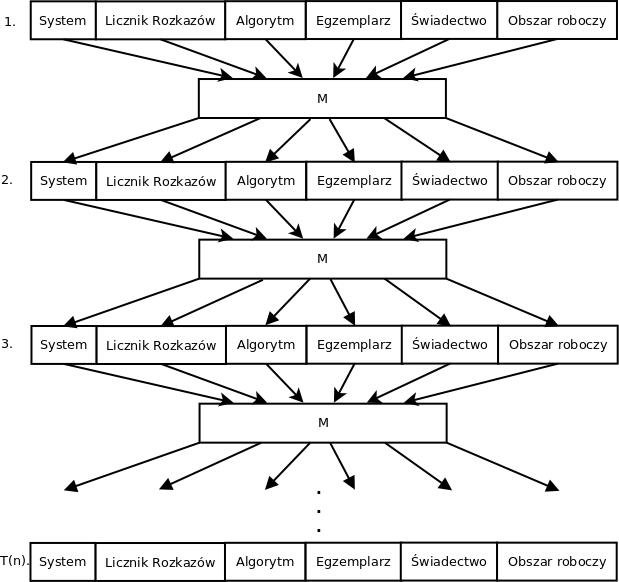
\includegraphics[width=0.75\hsize]{first_problem/configuration_sequence.png}
\caption{Sekwencja konfiguracji}
\label{configuration_sequence}
\end{figure}
\newpage
Zajmijmy się teraz sprawdzeniem czy problem spełnialności układów logicznych jest NP-trudny:

\begin{lem}
	CIRCUIT-SAT $\in$ NP-trudny.
\end{lem}

\begin{proof}
Aby wykazać, iż CIRCUIT-SAT jest NP-trudny pokażemy, że każdy problem z klasy NP można zredukować do CIRCUIT-SAT. W tym celu wyznaczymy kolejne etapy, które to przedstawią:

%\begin{enumerate}
%\item Zdefiniowanie algorytmu redukcji
%\item Analiza poprawności
%\item Analiza złożoności
%\item Podsumowanie
%\end{enumerate}

\begin{enumerate}
\item Zdefiniowanie algorytmu redukcji.

Dla każdego problemu $Q$ z klasy NP jesteśmy w stanie określić dwuparametrowy algorytm $A$, którego zadaniem jest zweryfikowanie świadectwa. W tym przypadku wykażemy zależność, iż jeśli świadectwo jest poprawne to można je przekształcić na odpowiednią postać binarną, która z kolei jest spełniającym wartościowaniem układu logicznego $C$. Również w drugą stronę, jeśli znajdziemy takie wartościowanie, które spełnia układ logiczny $C$ to będzie go można przeformułować na postać świadectwa które będzie poprawnie weryfikowane przez algorytm $A$.

Skupmy się teraz na konstrukcji która zamienia proces wykonywania algorytmu $A$ na tworzenie układu logicznego $C$. Jak wcześniej wspomniałem, wszystkie dane zawierające informacje na temat komputera i algorytmu $A$ znajdują się w pamięci komputera i wspólnie stanowią pierwszą konfiguracje. Następnie maszyna M przeprowadza kolejne kroki algorytmu, przechodząc z jednej konfiguracji w drugą, aż do momentu zakończenia działania algorytmu $A$. W rezultacie liczba konfiguracji jest dokładnie równa $T(n)$, czyli liczbie kroków jakie potrzebuje algorytm $A$ do uzyskania wyniku końcowego. Jak widać przez cały ten czas maszyna $M$ pozostaje niezmienna a jej postępowanie zależy jedynie od konfiguracji i przez ten czas jak będzie się zmieniała konfiguracja tak również maszyna $M$ będzie zmieniała różne obszary pamięci.
	
Aby sprowadzić zasadę działania wykonywania algorytmu $A$ w komputerze do struktury problemu CIRCUIT-SAT, to konfiguracja $c_{0}$ jest przewodami wejściowymi do układu logicznego. Następnie działa na to struktura logiczna maszyny $M$. W wyniku takiego działania otrzymujemy wyjście, które jest zapisywane jako konfiguracja $c_{1}$, jednak w naszym schemacie nie możemy zastosować takie rozwiązania w wyniku czego po prostu przedłużamy otrzymane ścieżki tak aby były kolejnym wejściem do powielonej maszyny $M$. Kontynuując to w ten sposób otrzymujemy tyle obszarów bramek logicznych ile wynosi liczba kroków algorytmu $A$. W końcowej fazie musimy wypuścić na wyjście ścieżkę z ostatniej konfiguracji $c_{T(n)}$ obszaru pamięci przeznaczonej na wynik algorytmu. Jest to wyjście naszego układu zawierającego odpowiedz na pytanie czy świadectwo jest prawdziwe. W ten oto sposób niejako "skleiliśmy" ze sobą przejścia przez wszystkie konfiguracje,tak by na końcu całego układu znalazła się końcowa konfiguracja $c_T(n)$.

\item Analiza poprawności

W ten sposób skonstruowany układ $C$, jak można zauważyć, jest spełnialny tylko wtedy gdy świadectwo jest pozytywnie zweryfikowane przez algorytm $A$, a nie może być inaczej gdyż układ $C$ symuluje obliczeniową naturę komputera. Z drugiej strony jeśli na wejście układu $C$ przedstawimy pewne wartościowanie które powoduje spełnialność układu oznacza, to że ta interpretacja binarna danych przekłada się na poprawne świadectwo, gdyż algorytm $A$ poprawnie weryfikuje to świadectwo, a jak wiemy $A$ jest poprawnym algorytmem. Zatem algorytm redukcji $F$ jest skonstruowany w sposób poprawny.

\item Analiza złożoności

Ostatnim elementem dowodu jest wykazanie wielomianowej złożoności algorytmu redukcyjnego $F$ względem rozmiaru danych wejściowych $n=|x|$. Niewątpliwie rozmiar potrzebny na dane związane ze stanem maszyny, obszarem licznika rozkazów i implementacją maszyny $M$ jest zależny od typu komputera który symuluje. Mimo to jest stały za względu na rozmiar danych przychodzących. Podobnie rozmiar algorytmu $A$ jest wartością stałą. Kolejnym czynnikiem są dane wejściowe egzemplarza $x$ oraz świadectwa $y$. Świadectwo będące podzbiorem egzemplarza jest nie większe rozmiarem od egzemplarza $x$, zaś rozmiar egzemplarza wynosi $n$. Ostatnim elementem przekładającym się na strukturze algorytmu $F$ jest obszar roboczy w którym znajdzie się wynik oraz który służy na pomocnicze obliczenia algorytmu złożoności wielomianowej $A$, czyli nie może być większy niż wielomianowa od rozmiaru danych. Zatem cała konstrukcja jednego kroku algorytmu redukcyjnego $F$ jest wielomianowa.

Teraz zwróćmy uwagę na liczbę kroków którą potrzebuje zrealizować algorytm $F$. Przypomnę że cała idea konstrukcji polega na symulowaniu działania algorytmu $A$ przez algorytm $F$. Zatem każda pojedyncza instrukcja algorytmu $A$ przekłada się na jeden wielomianowy krok algorytmu $F$. Skoro więc wielomian od wielomianu nadal jest wielomianem czyli całość działania algorytmu $F$ jest ostatecznie wielomianowa.
	
\item Podsumowanie

Podsumowując pokazaliśmy, że algorytm redukcji $F$ w poprawny sposób symuluje działanie każdego algorytmu dającego przedstawić się w strukturze komputerowej. Ponadto jeśli złożoność czasowa symulowanego algorytmu nie jest większa od wielomianowej to złożoność czasowa algorytmu redukcyjnego $F$ też jest wielomianowa. Oznacza to, że problem CIRCUIT-SAT jest tak samo trudny jak każdy problem należący do klasy NP, czyli CIRCUIT-SAT $\in$ NP-trudny.
\end{enumerate}
\end{proof}

\begin{twr}
	CIRCUIT-SAT $\in$ NP-zupełny
\end{twr}

\begin{proof}
Reasumując to że CIRCUIT-SAT $\in$ NP i CIRCUIT-SAT $\in$ NP-trudny otrzymujemy, że CIRCUIT-SAT $\in$ NP-zupełny.
\end{proof}

%\section{Podsumowanie}

Wynika z tego wniosek że o ile klasa NP-zupełna jest nie pusta (czyli ciągle nie rozstrzygnięte przez ludzkość pytanie czy NP $=$ P) to niewątpliwie CIRCUIT-SAT należy do tej klasy.
